\documentclass{article}
\usepackage[screen]{geometry}
\usepackage{alltt,xcolor}
\usepackage[utf8]{inputenc}
\usepackage{listings}
\usepackage{graphicx}
\lstset{escapechar=\@,language=C++,keywordstyle=\color{blue},showstringspaces=false}
\begin{document}
\large 
\section*{Specification}
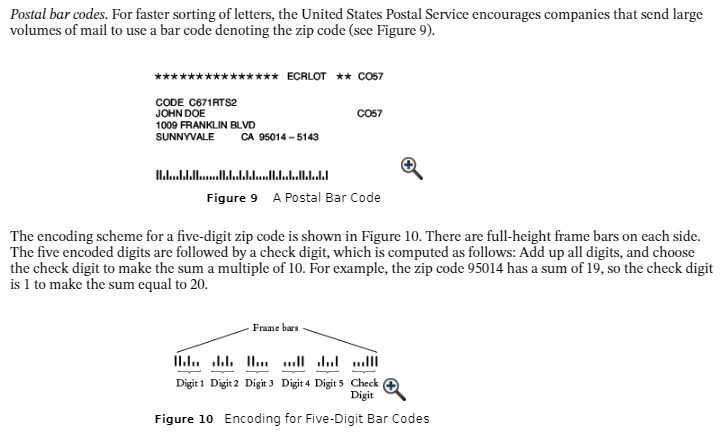
\includegraphics{postalBarCode1.png}
\newpage
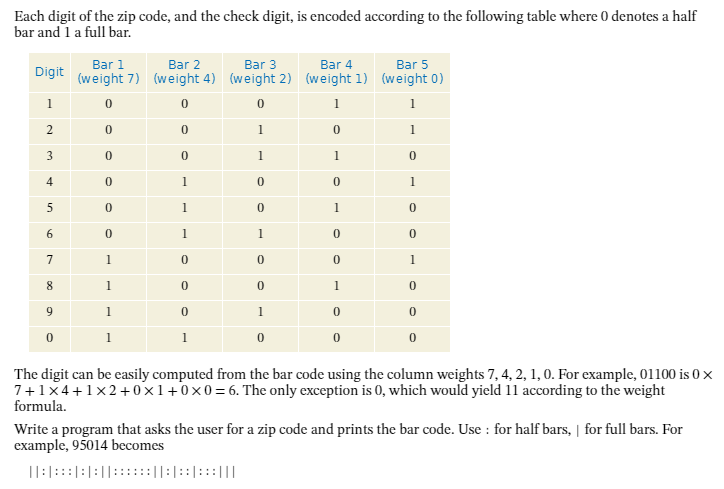
\includegraphics{postalBarCode2.png}
\newpage\section*{Analysis}
\begin{description}
	\item[Input] zipcode as a string in the \verb|QUERY_STRING| environment variable from the web server.
	\item[Preocess]Converts the zip code to the bar code.
	\item[Output] a bar code representing the zip code as a string 
	              of characters where $\vert$ represents the full bar
	              and : represents the half bar.
\end{description}
\newpage\section*{Design}
Functions needed:
\begin{itemize}
	\item compute check code: expects a zip code as string or integer(My input is a string at first ,but then I translate the string into an integer by using iss function), return either char of integer for the check digit.
	 The check digit is calculated by summing the five digits of the zip code and finding a digit that would bring the total to a number which is a multiple of 10.
	\item find bar code for zip code: given the zip code string or 
	integer (My input is a string at first ,but then I translate the string into an integer by using iss function)and returns the bar code delimited with full bars.
	\item find bar code for one digit: given a single digit, returns 
	the corresponding bar code.
\end{itemize}
\newpage\section*{Implementation}
\lstinputlisting{lab.cpp}
\lstinputlisting{lab4.html}
\newpage\section*{Test}
\subsection*{Testcase 1}
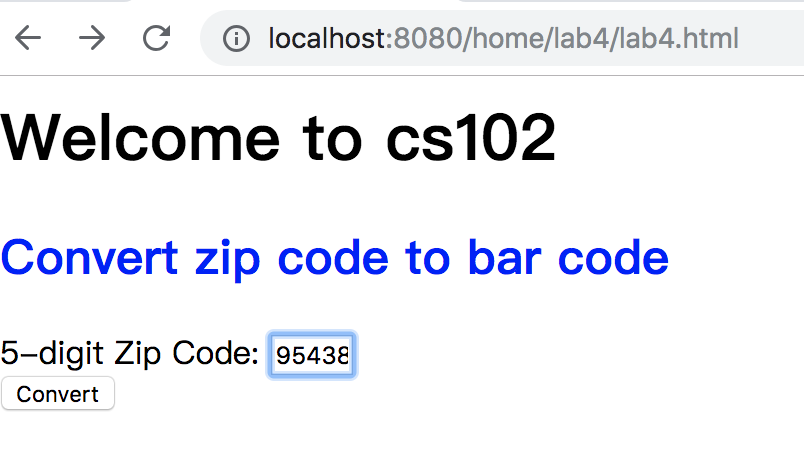
\includegraphics[width = 10cm, height = 6cm]{1.png}
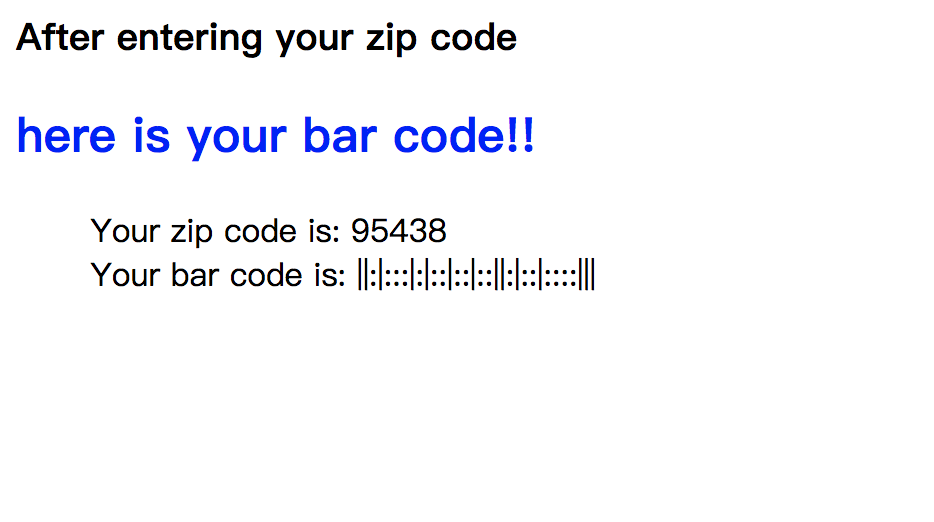
\includegraphics[width = 11cm, height = 6cm]{5.png}
Let's test it now! For example if user types in 95438, then program will display:

\verb-||:|:::|:|::|::|::||:|::|::::|||-

It proves that my code is correct!!It can exactly output the bar code.

\subsection*{Testcase 2}
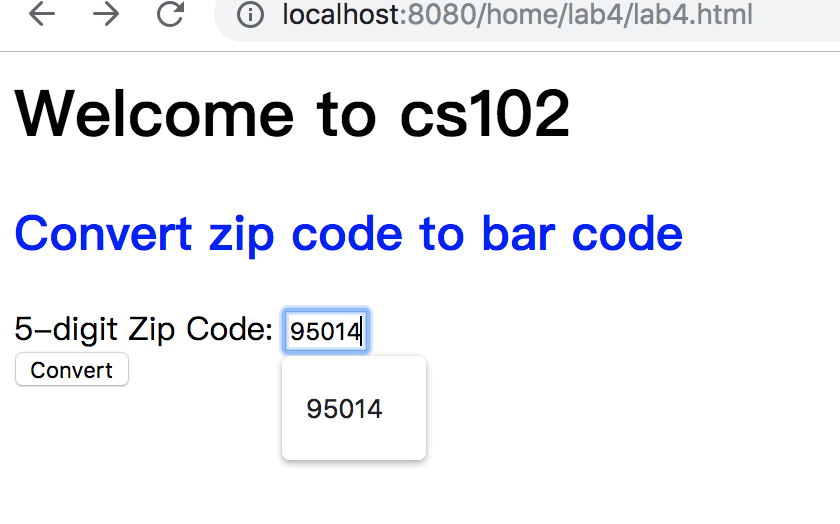
\includegraphics[width = 10cm, height = 6cm]{3.png}
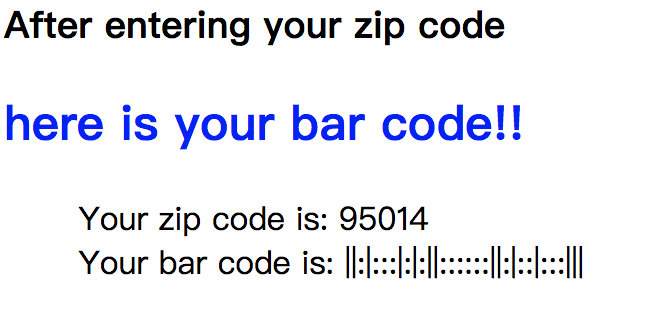
\includegraphics[width = 9cm, height = 4cm]{6.png}
For example if user types in 95014, then program will display:

\begin{verbatim}
	||:|:::|:|:||::::::||:|::|:::|||
\end{verbatim}
It also proves that my code is correct!!It can exactly output the bar code.

\end{document}
